\documentclass{standalone}
\usepackage{tikz}
\usepackage{ctex}
\setCJKmainfont{Noto Serif CJK SC}
\usepackage{mhchem,siunitx}
\begin{document}
\small
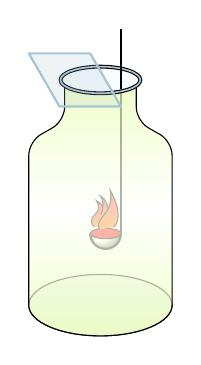
\begin{tikzpicture}[>=stealth,scale=1.3,inner sep=2pt]
  \draw[thick](0.2,0.9)--(0.2,-0.5);
  \draw[thick,ball color=white](0.2,-0.5)arc(0:-180:0.15);
  \draw[fill=red](0.05,-0.5)ellipse(0.15 and 0.05);
  \draw[fill=cyan!10!lightgray!20](0,-1.2)ellipse(0.7 and 0.3);
  \draw[top color=red!80!yellow,bottom color=orange](-0.061,-0.437)..controls(-0.157,-0.318)and( 0.046,-0.318)..
(-0.039,-0.180)..controls( 0.112,-0.264)and(-0.023,-0.373)..( 0.038,-0.425);
  \draw[top color=red!80!yellow,bottom color=orange]( 0.003,-0.317)..controls( 0.040,-0.240)and( 0.025,-0.162)..
(-0.001,-0.133)..controls( 0.071,-0.177)and( 0.093,-0.277)..( 0.075,-0.368);
  \draw[top color=red!80!yellow,bottom color=orange](-0.009,-0.462)..controls(-0.064,-0.329)and( 0.139,-0.329)..
( 0.095,-0.077)..controls( 0.205,-0.275)and( 0.181,-0.390)..( 0.131,-0.436);
  
  \draw[rounded corners=5pt,top color=green!30!yellow!30,bottom color=green!30!yellow!30,middle color=white,fill opacity=0.7](0.35,1.0)--(0.35,0.6)--(0.7,0.4)[sharp corners]--(0.7,-1.2)arc(0:-180:0.7 and 0.3)[rounded corners=5pt]--(-0.7,0.4)--(-0.35,0.6)--(-0.35,1.0);
  \draw[double=cyan!20!lightgray,fill=cyan!3](0,1.0)ellipse(0.39 and 0.13);
  \draw[thick](0.2,0.91)--(0.2,1.5);
  \draw[thick,cyan!20!lightgray,line join =round,fill=cyan!20!lightgray,fill opacity=0.2](0.05,1)--++(-60:0.3)--++(-0.6,0)--++(120:0.6)--++(0.6,0)--cycle;
\end{tikzpicture}
\end{document}